\documentclass[spanish]{udpreport}
\usepackage[utf8]{inputenc}
\usepackage[spanish]{babel}
\usepackage{graphicx}
\usepackage{float}
\usepackage{etoolbox,fancyhdr,xcolor}
% Podemos establecer el logo de alguna entidad o dejar el de la UDP (defecto)
%\setlogo{EITFI}



\title{Informe de laboratorio numero 5}
\pagestyle{fancy} %coloca el entorno para encabezado y pie de página
\headheight=3pt %para cambiar el tamaño del encabezado
\rhead{\bfseries } %solo aparce lo que nosostros coloquemos
\fancyhead[C] %la "L" indica a la izquierda
{
Ingenieria civil Informatica y Telecomunicaciones
}

\begin{document}


  \author{Alumnos:	Thomas Gonzáles\linebreak Michiru Nakamura\linebreak Flavio Pallini\linebreak Fernando Peña\linebreak\linebreak Profesor:	Jaime Álvarez \linebreak Ayudante:	Maximiliano Vega }

\email{fernando.Penas@mail.udp.cl\linebreak thomas.gonzalez@mail.udp.cl \linebreak michiru.nakamura@mail.udp.cl\linebreak Flavio.pallini@mail.udp.cl }
\date{07 de Julio de 2016}

% Además podemos establecer la facultad y escuela
% los valores por defecto son los siguientes:
%\udpschool{Escuela de Informática y Telecomunicaciones}
%\udpfaculty{Facultad de Ingeniería}
%\udpuniversity{Universidad Diego Portales}


\maketitle

\tableofcontents

\chapter{Introducción}
\LARGE El ruteo (también denominado enrutamiento, encaminamiento, o \textit{routing}) es el procedimiento por el cual un dispositivo elige de entre un número de rutas posibles, la mejor. Cómo se determina la mejor ruta dependerá de cómo se defina ésta, según características como longitud de la ruta, su disponibilidad, su fiabilidad, entre otras. En redes informáticas, se hablará de ruteo con respecto al envío de datagramas por medio de los enlaces de red. \\

Existen varios protocolos de ruteo que utilizan distintas exigencias de red y consideran diferentes características para su trabajo. En esta experiencia se estudió el ruteo estático y el ruteo por RIP.
\noindent

\chapter{Configuración de la red}

Utilizándose el \textit{Packet Tracer} de Cisco, se configuró una red virtual de cuatro routers, donde cada router se conectó a sus dos routers adyacentes y a un switch, este último conectado a dos computadores terminales.

\begin{figure}[H]
	\begin{center}
		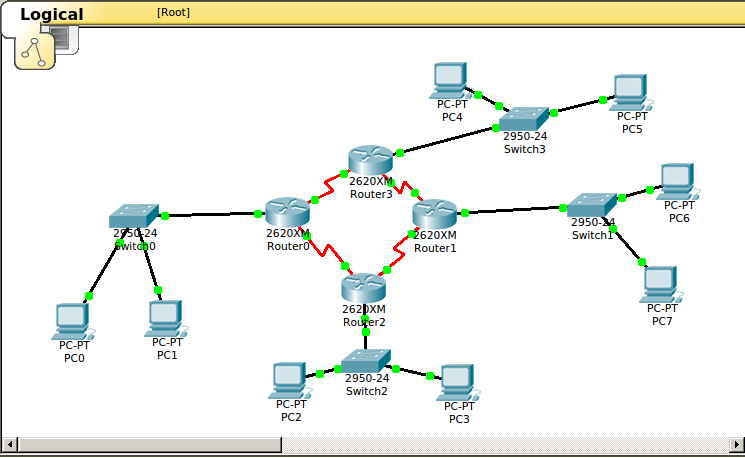
\includegraphics[width= 17cm]{Imagenes/red_pela}
		\caption{Red virtual utilizada en ambas experiencias.}
	\end{center}
\end{figure}

Se configuraron las direcciones IP de cada dispositivo asignándole a cada subred su propia dirección de clase C.

\begin{figure}[H]
	\begin{center}
    	\begin{tabular}{ c | c | c }
        	\textbf{Tipo de Red} & \textbf{\textit{Router}(s) conectados} & \textbf{Nombre de red}\\
            \hline
            LAN & \textit{Router} 0 & 10.0.0.0 \\
            LAN & \textit{Router} 1 & 10.0.1.0 \\
            LAN & \textit{Router} 2 & 10.0.2.0 \\
            LAN & \textit{Router} 3 & 10.0.3.0 \\
            WAN & \textit{Routers} 0 y 3 & 10.0.4.0 \\
            WAN & \textit{Routers} 1 y 2 & 10.0.5.0 \\
            WAN & \textit{Routers} 2 y 0 & 10.0.6.0 \\
            WAN & \textit{Routers }3 y 1 & 10.0.7.0 \\
        \end{tabular}
        \caption{Tabla de direcciones de red}
	\end{center}
\end{figure}

Para hacer esto, en primer lugar se configuró la conexión\textit{ Fast Ethernet }de cada \textit{router} con su IP LAN, estableciéndose la dirección .1 como \textit{gateway} y las direcciones .2 y .3 para los dispositivos terminales.\\

\begin{figure}[H]
	\begin{center}
		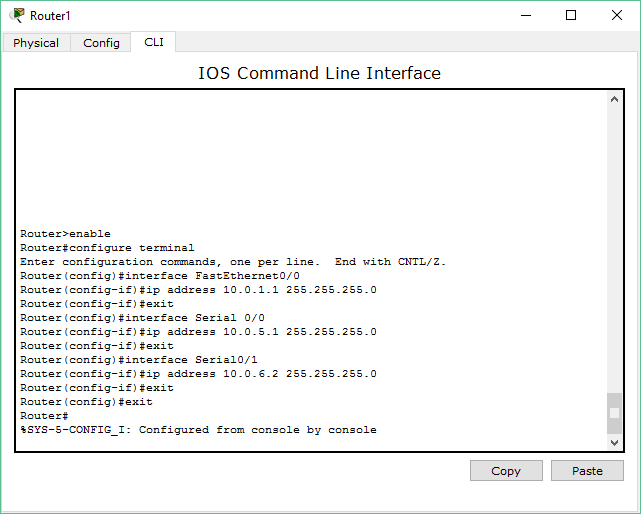
\includegraphics[width= 12.5cm]{Imagenes/configuracion_IPs}
		\caption{Asignación de las direcciones del \textit{router}.}
	\end{center}
\end{figure}

\begin{figure}[H]
	\begin{center}
		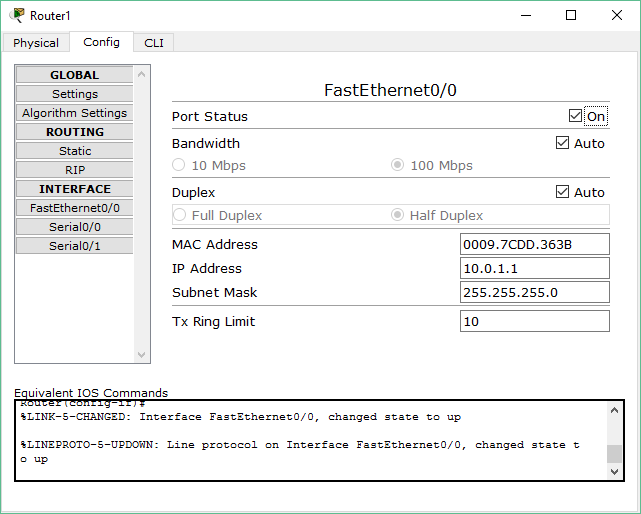
\includegraphics[width= 12.5cm]{Imagenes/FE0}
		\caption{Dirección \textit{Fast Ethernet} del \textit{router} 1.}
	\end{center}
\end{figure}

\begin{figure}[H]
	\begin{center}
		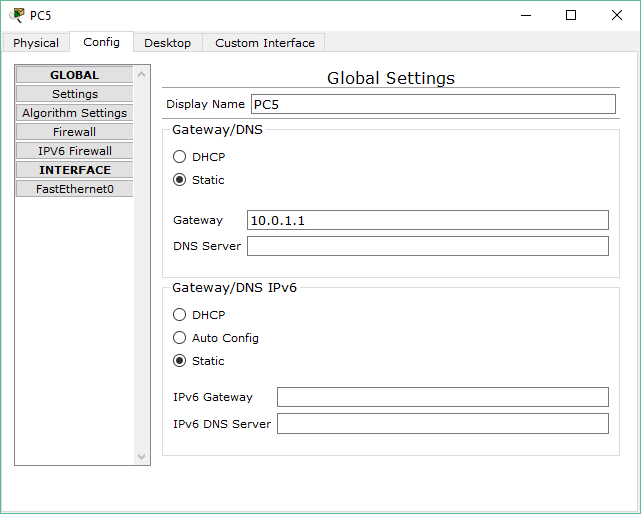
\includegraphics[width= 12cm]{Imagenes/gateway_PC5}
		\caption{Configuración del \textit{router} 1 como \textit{gateway} de la red 1.}
	\end{center}
\end{figure}

\begin{figure}[H]
	\begin{center}
		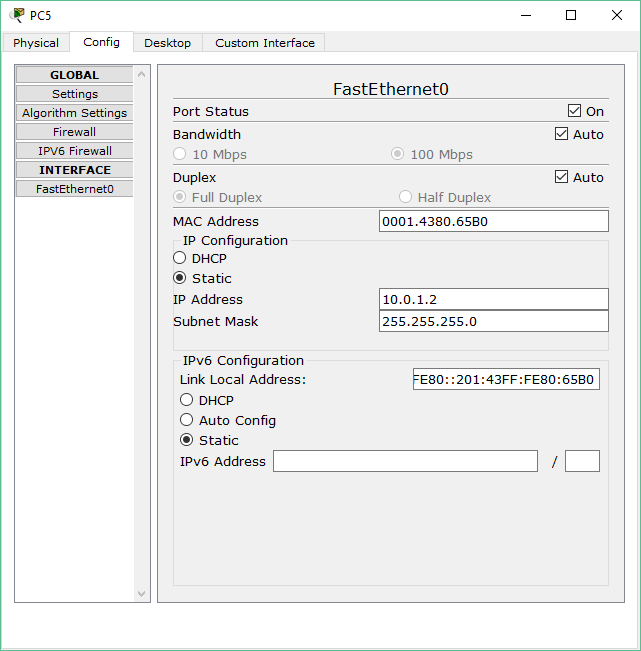
\includegraphics[width= 12cm]{Imagenes/IP_PC5}
		\caption{Configuración de la dirección y máscara propios de este dispositivo.}
	\end{center}
\end{figure}

Hecho esto, se debió especificar las direcciones de cada enlace serial utilizándose las direcciones de sus respectivas redes WAN.

\begin{figure}[H]
	\begin{center}
		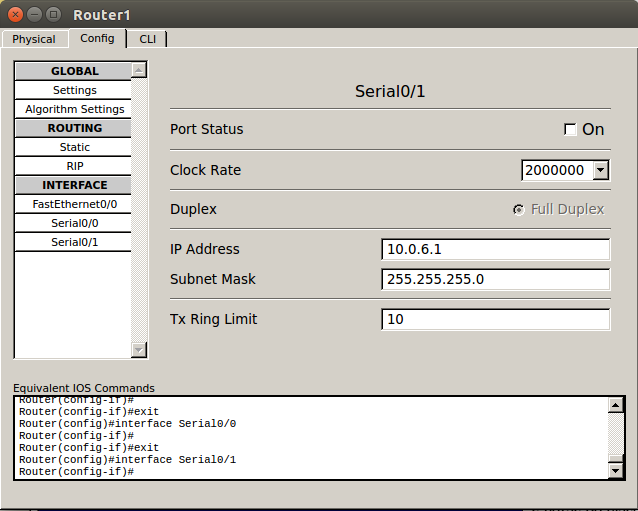
\includegraphics[width= 12cm]{Imagenes/serial2}
		\caption{Configuración de un enlace serial del \textit{router} 1, dirigido al \textit{router} 2.}
	\end{center}
\end{figure}

\begin{figure}[H]
	\begin{center}
		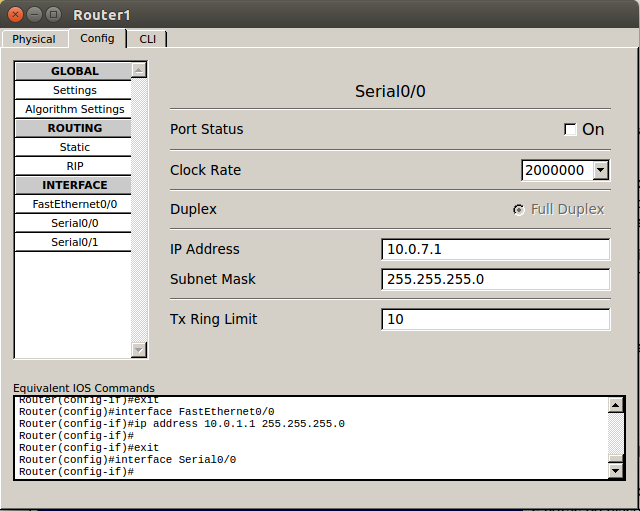
\includegraphics[width= 12cm]{Imagenes/serial1}
		\caption{Configuración del otro enlace serial del \textit{router} 1, dirigido al\textit{ router} 3.}
	\end{center}
\end{figure}


\chapter{Ruteo Estatico}

Ruteo estático quiere decir que cada red tiene un enlace preestablecido por el cuál se va a dirigir, por lo que es necesario ahora designar dichas rutas en la interfaz de líneas de comando, usándose el comando \textit{ip route} seguido de la red LAN de destino, su máscara de red, y el enlace WAN a utilizarse. \\

Para las redes adyacentes, naturalmente se configuró tal que los enlaces WAN correspondieran a las redes LAN asociadas al mismo router, mientras que para la red opuesta al no existir un enlace directo se estableció que el paquete fuera enviado al enlace WAN a su izquierda como paso intermedio a su red de destino.

\begin{figure}[H]
	\begin{center}
		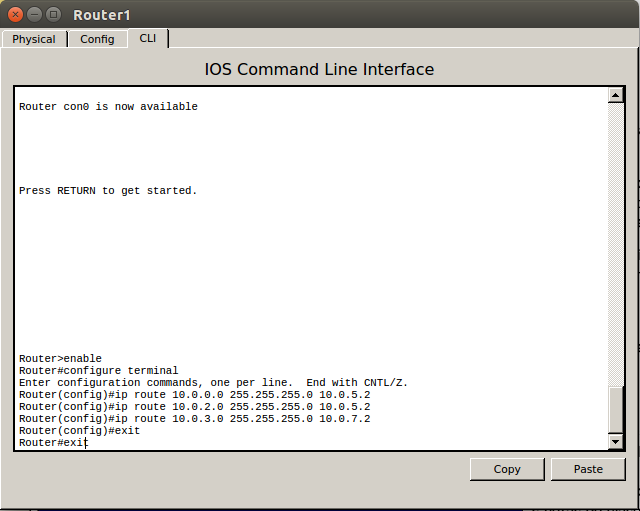
\includegraphics[width= 17cm]{Imagenes/config_estatico}
		\caption{Configuración de las rutas del \textit{Router} 1.}
	\end{center}
\end{figure}

Estando el sistema configurado por completo, se probó enviar un paquete desde el PC 7 hacia el PC 1, el primero en la red LAN 1 y el segundo en la red LAN 0 opuesta.

\begin{figure}[H]
	\begin{center}
		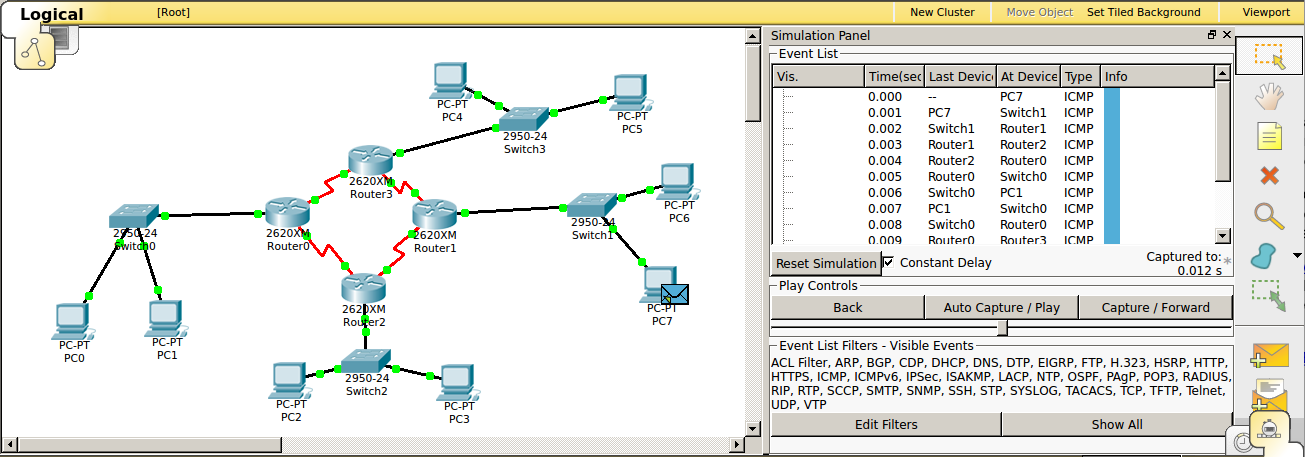
\includegraphics[width= 17cm]{Imagenes/envio_estatico}
		\caption{Imagen de la red con el registro de envío de paquetes.}
	\end{center}
\end{figure}

Se ve en la figura que el paquete se dirigió en primer lugar a su \textit{router gateway}, para luego seguir los enlaces WAN hacia el router 2 y el router 0, para finalmente ingresar a la red y ser recibido por el PC 1. Luego, este PC envió un paquete \textit{acknowledge} de vuelta, pasando por el router 3 antes de pasar por el router 0, comprobándose que todo paquete seguirá sólo la ruta preestablecida hacia su objetivo. Y, si bien no se alcanza a apreciar en el registro de envío, este \textit{acknowledge} fue recibido sin problemas por el PC 7. Quedan comprobadas la funcionalidad y eficiencia de la red.

Cabe destacar que, de haberse configurado este sistema de forma práctica, hubiera sido necesario configurar una ruta por defecto para todo paquete encaminado fuera de las direcciones establecidas en la lista de rutas. Éste normalmente sería un paquete encaminado hacia la Internet, o cuando mínimo a una red WAN ajena a la del sistema.

\chapter{Ruteo dinamico}

Ruteo dinámico quiere decir que existe un cambio constante en las rutas preferidas para acceder a alguna red, en base a diversas características. En el RIP (\textit{Routing Information Protocol}, Protocolo de Información de Ruteo) el factor decisivo para elegir una ruta es la cantidad de saltos a realizarse para enviar un paquete a su destino, para los enlaces establecidos en su última verificación.

Trabajándose desde la misma red anterior pero eliminando cualquier configuración relacionada a ruteo estático, se procedió a configurar RIP. Para ello, en la interfaz de líneas de comando se utilizó el comando \textit{router rip} con la dirección de la red a la que conecta el router.

\begin{figure}[H]
	\begin{center}
		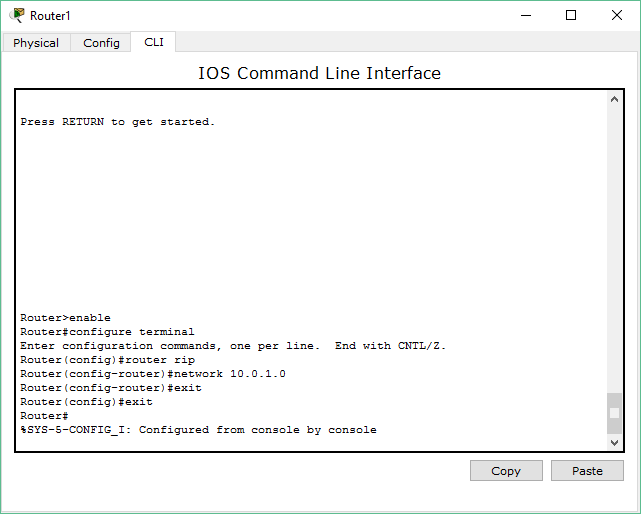
\includegraphics[width= 17cm]{Imagenes/config_rip}
		\caption{Configuración del RIP del \textit{router} 1.}
	\end{center}
\end{figure}

Una vez hecho esto para cada \textit{router}, se procedió a enviar un paquete desde el PC 7 al PC 0, el primero en la red LAN 3 y el segundo en la red LAN 0, adyacentes.

\begin{figure}[H]
	\begin{center}
		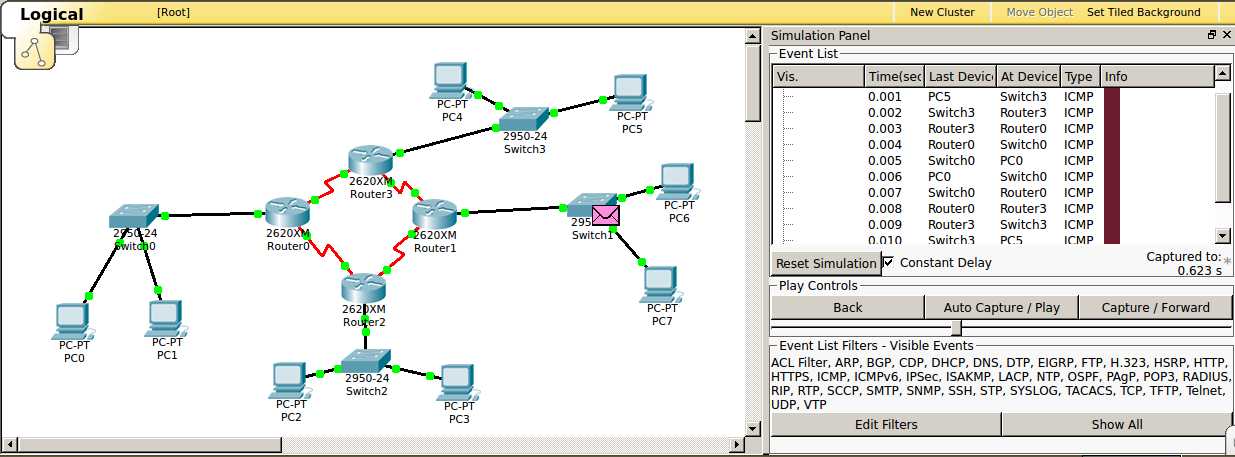
\includegraphics[width= 17cm]{Imagenes/envio_rip}
		\caption{Imagen de la red con el registro de envío de paquetes.}
	\end{center}
\end{figure}

Se ve del registro que el paquete poseía dos rutas para ser enviado: una sin saltos, y una con dos saltos. Naturalmente, el paquete fue enviado por la ruta sin saltos y recibido sin problemas, para luego enviar un \textit{acknowledge} de vuelta. Se nota que en ningún momento se le hizo explícito a los \textit{routers} hacia dónde se dirigía cada enlace más alla de las configuraciones WAN, calculando éstos la ruta más óptima periódicamente.

\chapter{Conclusión}
El ruteo estático puede ser eficiente y preciso al ser establecido manualmente por parte del encargado de la red en redes de tamaño pequeño, tales como la red de una PyME, pues configurarlo manualmente no requiere mucho trabajo y además se evita el envio constante de información de ruteo a través de la red utilizado por los protocolos de ruteo, haciendo la red más expedita. Sin embargo para redes de tamaño considerable, como lo sería la red de una empresa de mayor tamaño, como un ISP, configurar los routers para enrutar estáticamente se vuelve algo complicado y requiere bastante tiempo y recursos, sin mencionar que la caída de un enlace podría potencialmente causar estragos. %Agregué "como un ISP" porque me acordé que el profe dijo en clases que para la mayoría de las empresas una red "pequeña" es suficiente para cubrir sus necesidades, así que pensé que podría ser útil decir qué red se consideraría "grande."

Por otro lado, el ruteo dinámico funciona muy bien en redes de gran tamaño al ser eficiente y automatizado. Al ser automatizado, el administrador de la red solo deberá configurar una dirección de ruteo para su red local, para que el protocolo haga su trabajo de forma automática actualizando constantemente las vias de ruteo, y por lo tanto haciendo que la red no requiera de mantención en términos de caminos, lo que lo convierte en el candidato más óptimo en la mayoría de los casos.

 \LARGE 
\noindent
\listoffigures

\end{document}